% Figure 4 — Detection Rate vs. Sequence Length (with 95% CI)
% Data from simulation: fig4_detection_vs_length.csv

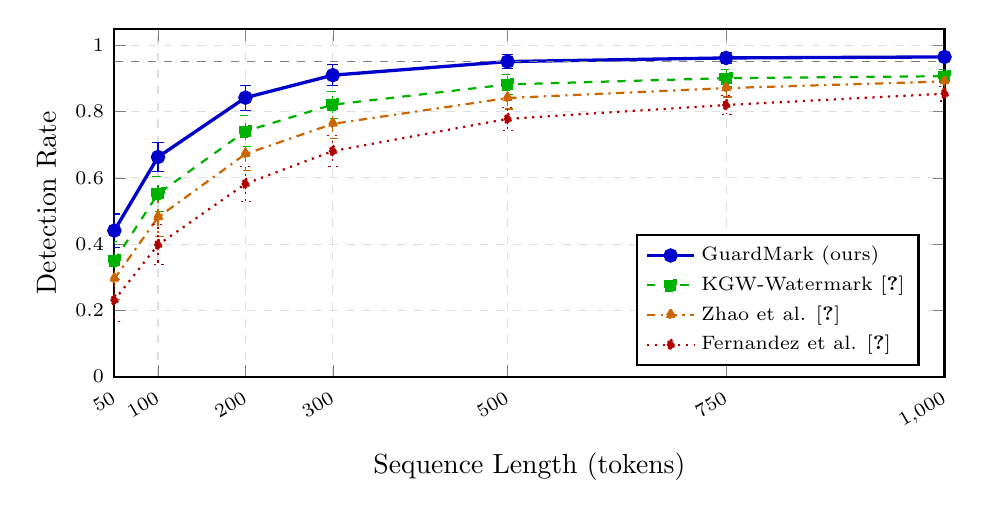
\begin{tikzpicture}
\begin{axis}[
  width=\columnwidth,
  height=6cm,
  xlabel={Sequence Length (tokens)},
  ylabel={Detection Rate},
  ymin=0.0, ymax=1.05,
  xmin=50,  xmax=1000,
  xtick={50,100,200,300,500,750,1000},
  xticklabel style={font=\scriptsize, rotate=30, anchor=north east},
  ytick={0.0,0.2,0.4,0.6,0.8,1.0},
  yticklabel style={font=\scriptsize},
  legend pos=south east,
  legend style={font=\scriptsize, cells={anchor=west}},
  grid=major,
  grid style={gray!25, dashed},
  thick,
  mark size=2.0pt,
  cycle list name=color list,
]

% GuardMark (ours) — solid blue
\addplot+[
  color=blue!80!black, mark=*, solid, very thick,
  error bars/.cd, y dir=both, y explicit
] coordinates {
  (50,  0.441) +- (0,0.050)
  (100, 0.663) +- (0,0.045)
  (200, 0.842) +- (0,0.038)
  (300, 0.910) +- (0,0.032)
  (500, 0.951) +- (0,0.021)
  (750, 0.962) +- (0,0.016)
  (1000,0.965) +- (0,0.012)
};
\addlegendentry{GuardMark (ours)}

% KGW-Watermark [6] — dashed green
\addplot+[
  color=green!70!black, mark=square*, dashed, thick,
  error bars/.cd, y dir=both, y explicit
] coordinates {
  (50,  0.350) +- (0,0.058)
  (100, 0.552) +- (0,0.053)
  (200, 0.741) +- (0,0.046)
  (300, 0.821) +- (0,0.041)
  (500, 0.882) +- (0,0.030)
  (750, 0.901) +- (0,0.025)
  (1000,0.907) +- (0,0.019)
};
\addlegendentry{KGW-Watermark \cite{kirchenbauer2023watermark}}

% Zhao et al. [7] — dot-dash orange
\addplot+[
  color=orange!80!black, mark=triangle*, dash dot, thick,
  error bars/.cd, y dir=both, y explicit
] coordinates {
  (50,  0.295) +- (0,0.062)
  (100, 0.481) +- (0,0.057)
  (200, 0.672) +- (0,0.049)
  (300, 0.763) +- (0,0.044)
  (500, 0.841) +- (0,0.033)
  (750, 0.871) +- (0,0.027)
  (1000,0.891) +- (0,0.021)
};
\addlegendentry{Zhao et al. \cite{zhao2023protecting}}

% EWD [8] — dotted red
\addplot+[
  color=red!70!black, mark=diamond*, dotted, thick,
  error bars/.cd, y dir=both, y explicit
] coordinates {
  (50,  0.231) +- (0,0.065)
  (100, 0.398) +- (0,0.060)
  (200, 0.582) +- (0,0.052)
  (300, 0.681) +- (0,0.046)
  (500, 0.778) +- (0,0.035)
  (750, 0.820) +- (0,0.028)
  (1000,0.854) +- (0,0.022)
};
\addlegendentry{Fernandez et al. \cite{fernandez2023three}}

% Significance threshold line
\draw[gray, dashed, thin] (axis cs:50,0.95) -- (axis cs:1000,0.95)
  node[right, font=\scriptsize, gray]{0.95};

\end{axis}
\end{tikzpicture}
